{
	\section{Определение графа. Смежность. Диаграммы. Псевдо-, гипер- и мультиграфы. Виды
графов. Связность}

\subsection*{Основное определение}

\textbf{Графом} $G(V, E)$ называется совокупность двух множеств — непустого множества $V$ (множества вершин) и множества $E$ двухэлементных подмножеств множества $V$ ($E$ — множество рёбер),


\[
G(V, E) \overset{\text{def}}{=} \langle V; E \rangle,\quad V \neq \emptyset,\quad E \subseteq 2^V\ \&\ \forall e \in E\ (|e| = 2).
\]

\subsection*{Смежность}

Пусть $v_1, v_2$ — вершины, $e = (v_1, v_2)$ — соединяющее их ребро. Тогда вершина $v_1$ и ребро $e$ \subsection*{7.1.3. Смежность}

Пусть $v_1, v_2$ — вершины, $e = (v_1, v_2)$ — соединяющее их ребро. Тогда вершина $v_1$ и ребро $e$ \textbf{инцидентны}, ребро $e$ и вершина $v_2$ также инцидентны. Два ребра, инцидентные одной вершине, называются \text{смежными}; две вершины, инцидентные одному ребру, также называются смежными.

Множество вершин, смежных с вершиной $v$, называется \textbf{множеством смежности} (или \textbf{окрестностью}) вершины $v$ и обозначается $\Gamma^+(v)$:


\[
\Gamma^+(v) \overset{\text{Def}}{=} \{ u \in V \mid (u, v) \in E \}, \quad \Gamma^*(v) \overset{\text{Def}}{=} \Gamma^+(v) + v.
\]



\paragraph{ЗАМЕЧАНИЕ.}
Если не оговорено противное, то символ $\Gamma$ без индекса подразумевает $\Gamma^+$, то есть саму вершину в окрестность не включают. \\

Очевидно, что $u \in \Gamma(v) \iff v \in \Gamma(u)$. Если $A \subset V$ — множество вершин, то $\Gamma(A)$ — множество всех вершин, смежных с вершинами из $A$:


\[
\Gamma(A) \overset{\text{Def}}{=} \{ u \in V \mid \exists \, v \in A\ (u \in \Gamma(v)) \} = \bigcup_{v \in A} \Gamma(v).
\]

\subsection*{Диаграммы}

Обычно граф изображают диаграммой: вершины — точками (или кружками), рёбра — линиями.

\textbf{Пример.} На рис.~7.4 приведён пример диаграммы графа, имеющего четыре вершины и пять рёбер.
В этом графе вершины $v_1$ и $v_2$, $v_2$ и $v_3$, $v_3$ и $v_4$, $v_4$ и $v_1$, $v_2$ и $v_4$ смежны, а вершины $v_1$ и $v_3$ не смежны.
Смежные рёбра: $e_1$ и $e_2$, $e_2$ и $e_3$, $e_3$ и $e_4$, $e_4$ и $e_1$, $e_1$ и $e_5$, $e_2$ и $e_5$, $e_3$ и $e_5$, $e_4$ и $e_5$.
Несмежные рёбра: $e_1$ и $e_3$, $e_2$ и $e_4$.

\begin{figure}[h]
  \centering
  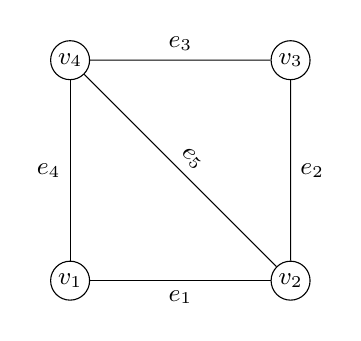
\begin{tikzpicture}[scale=1.4, every node/.style={font=\small}]
    % вершины
    \node[circle, draw, inner sep=1.5pt] (v1) at (0,0) {$v_1$};
    \node[circle, draw, inner sep=1.5pt] (v2) at (2,0) {$v_2$};
    \node[circle, draw, inner sep=1.5pt] (v3) at (2,2) {$v_3$};
    \node[circle, draw, inner sep=1.5pt] (v4) at (0,2) {$v_4$};

    % рёбра
    \draw (v1) -- (v2) node[midway, below] {$e_1$};
    \draw (v2) -- (v3) node[midway, right] {$e_2$};
    \draw (v3) -- (v4) node[midway, above] {$e_3$};
    \draw (v4) -- (v1) node[midway, left] {$e_4$};
    \draw (v2) -- (v4) node[midway, sloped, above] {$e_5$};
  \end{tikzpicture}
  \caption{Диаграмма графа}
\end{figure}

\subsection*{Типы графов}

\begin{enumerate}
    \item \textbf{Псевдограф} — граф с петлями.
    \item \textbf{Мультиграф} — граф с кратными рёбрами.
    \item \textbf{Гиперграф} — дуги являются множествами с одним и более элементами.
    \item \textbf{Нумерованный граф} — если существует функция, отображающая множество вершин или рёбер в множество чисел или символов.
\end{enumerate}

\begin{itemize}
    \item Если элементом множества $E$ может быть пара одинаковых (не различных) элементов $V$, то такой элемент называется \textbf{петлёй}, а граф — \textbf{графом с петлями} (или \textbf{псевдографом}).
    \item Если $E$ является не множеством, а мультимножеством, содержащим некоторые элементы по несколько раз, то такие элементы называются \textbf{кратными рёбрами}, а граф — \textbf{мультиграфом}.
    \item Если элементами множества $E$ являются не обязательно двузначные, а любые (непустые) подмножества множества $V$, то такие элементы называются \textbf{гипердугами}, а граф — \textbf{гиперграфом}.
    \item Если задана функция $F: V \to M$ и/или $F: E \to M$, то множество $M$ называется \textbf{множеством пометок}, а граф — \textbf{помеченным} (или \textbf{нагруженным}). В качестве множества пометок обычно используются буквы или целые числа. Если функция $F$ инъективна, то есть разные вершины (рёбра) имеют разные пометки, то граф называют \textbf{нумерованным}.
\end{itemize}

\subsection*{Специальные графы}

\begin{itemize}
    \item \textbf{Тривиальный граф} — состоит из одной вершины.
    \item \textbf{Циклический граф с $k$ вершинами} — обозначается $C_k$.
    \item \textbf{Полный граф} — содержит все возможные рёбра между вершинами, обозначается $K_p$.
\end{itemize}

Число рёбер в полном графе:


\[
q(K_p) = \frac{p(p - 1)}{2}.
\]



\subsection*{Колёса и двудольные графы}

\begin{itemize}
    \item \textbf{Колесо} — граф, обозначаемый $W_n$.
    \item \textbf{Двудольный граф} — граф, множество вершин $V$ которого можно разбить на два непересекающихся множества $V_1$ и $V_2$ так, что каждое ребро из $E$ инцидентно вершинам из $V_1$ и $V_2$. Множества $V_1$ и $V_2$ называются \textbf{долями графа}.
\end{itemize}

\subsection*{Связность графа}

Говорят, что две вершины в графе \textbf{связаны}, если существует соединяющая их (простая) цепь. Граф, в котором все вершины связны, называется \textbf{связным}.

Связность является \textbf{эквивалентностью}. Классы эквивалентности по отношению связности — это \textbf{компоненты связности} графа:


\[
k(G).
\]



Граф, состоящий только из вершин, называется \textbf{вполне несвязным}.


	\newpage
}
